% Asset ID: A21AlgebraicMethodsProofByContradictionTikZ-001
% Source: CCEA proof and reasoning theme; teacher transcript; Phase 1 Core Theory
% Related lesson section: Core Theory
% Purpose: Show the formal proof-by-contradiction loop.
\documentclass[tikz,border=8pt]{standalone}
\usepackage{amsmath}
\usetikzlibrary{arrows.meta,positioning}
\begin{document}
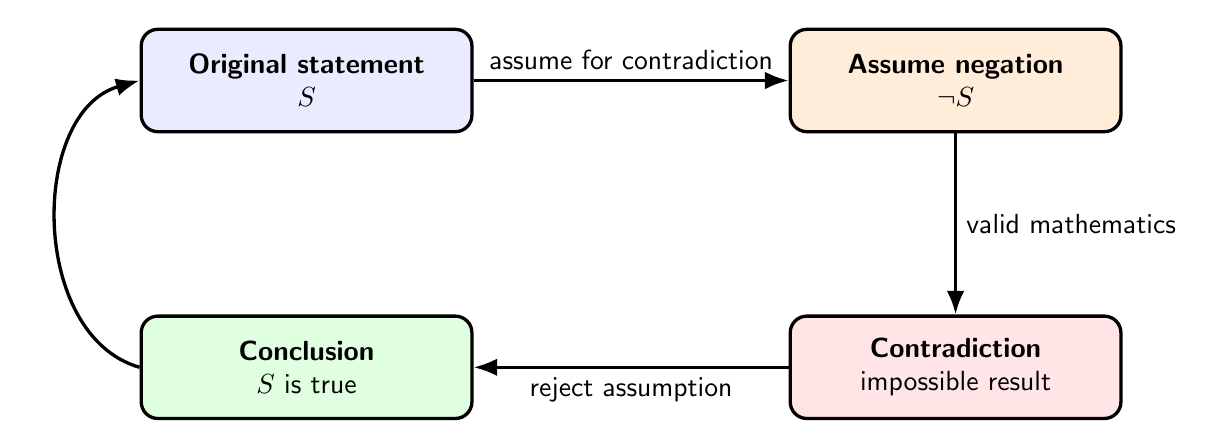
\begin{tikzpicture}[font=\sffamily, box/.style={rectangle, rounded corners=6pt, draw=black, very thick, align=center, minimum width=4.2cm, minimum height=1.3cm}, arrow/.style={-{Latex[length=3mm]}, very thick}]
\node[box, fill=blue!8] (S) {\textbf{Original statement}\\ $S$};
\node[box, fill=orange!15, right=4cm of S] (notS) {\textbf{Assume negation}\\ $\neg S$};
\node[box, fill=red!10, below=2.3cm of notS] (contradiction) {\textbf{Contradiction}\\ impossible result};
\node[box, fill=green!12, below=2.3cm of S] (conclusion) {\textbf{Conclusion}\\ $S$ is true};
\draw[arrow] (S) -- node[above]{assume for contradiction} (notS);
\draw[arrow] (notS) -- node[right]{valid mathematics} (contradiction);
\draw[arrow] (contradiction) -- node[below]{reject assumption} (conclusion);
\draw[arrow] (conclusion.west) .. controls +(-1.4,0.4) and +(-1.4,-0.4) .. (S.west);
\end{tikzpicture}
\end{document}
